\section{Kết Quả Thực Nghiệm và Phân Tích Chuyên Sâu}

\subsection{Thống kê chuẩn hóa cấu trúc và kiểm toán toàn cục hai tập ngữ liệu}

Sau khi hoàn tất các bước khử trang quét đúp, xoay phục hồi trang ngược, tái ghép tay sách bị hoán vị và đối chiếu đồng bộ tự động giữa ảnh, nhãn hộp tọa độ, nhãn ký tự đơn và bảng dóng hàng, toàn bộ cấu trúc và các chỉ số chất lượng của hai tập ngữ liệu được tổng hợp trong Bảng~\ref{tab:corpus_stats}. Cả hai tập đều được khai báo thống nhất là \textbf{bản dịch âm 1--1} trên toàn bộ chính văn, không có phân đoạn dịch nghĩa nên số hàng không so sánh (\texttt{null}) bằng $0$ ($0{,}00\%$) trên tổng số $5.096$ cặp câu. Trong suốt quy trình xây dựng, hệ thống cũng không sử dụng cơ chế gợi ý chữ Nôm tự động từ nguồn thay thế hay nguồn tự hình tương tự, do đó số gợi ý được chấp nhận và số gợi ý bị bác bỏ đều bằng $0$.

\begin{table}[H]
    \centering
    \footnotesize
    \renewcommand{\arraystretch}{1.22}
    \begin{tabularx}{\textwidth}{X c c c}
        \toprule
        \textbf{Chỉ số cấu trúc và kiểm toán ngữ liệu} & \textbf{Tập 1} & \textbf{Tập 2} & \textbf{Tổng cộng} \\
        \midrule
        Số trang quét nguyên bản đầu vào & $636$ & $685$ & $1.321$ \\
        Số trang hiệu lực sau khử trùng lặp & $636$ & $683$ (loại $27, 28$) & $\mathbf{1.319}$ \\
        Số trang Quốc ngữ / Hán Nôm chính văn & $303 \;/\; 305$ & $331 \;/\; 331$ & $\mathbf{634 \;/\; 636}$ \\
        Số trang Nôm khuyết bản Quốc ngữ đối ứng & $2$ (trang $358, 359$) & $0$ & $\mathbf{2}$ \\
        Trang phụ trợ (Lời tựa / Chú thích / Mục lục) & $4 \;/\; 1 \;/\; 7$ & $0 \;/\; 1 \;/\; 7$ & $4 \;/\; 2 \;/\; 14$ \\
        Trang không nội dung (Trang trắng / Bìa \& khác) & $10 \;/\; 6$ & $8 \;/\; 5$ & $18 \;/\; 11$ \\
        Số trang quét ngược $180^\circ$ đã phục hồi & $1$ (trang $421$) & $3$ ($453, 485, 521$) & $\mathbf{4}$ \\
        Số trang Nôm đóng sai vị trí đã tái ghép & $4$ ($581/582, 591/592$) & $0$ & $\mathbf{4}$ \\
        Tổng số đơn vị ánh xạ trang chính văn & $305$ ($303$ cặp $+ 2$) & $331$ (1--1 toàn phần) & $\mathbf{636}$ \\
        \midrule
        Tổng số cặp câu song ngữ 1--1 & $2.141$ & $2.955$ & $\mathbf{5.096}$ \\
        Số hàng không so sánh (tỷ lệ hàng \texttt{null}) & $0$ ($0{,}00\%$) & $0$ ($0{,}00\%$) & $\mathbf{0\;(0{,}00\%)}$ \\
        Tổng số tự hình Hán Nôm trên toàn tập & $69.586$ & $76.691$ & $\mathbf{146.277}$ \\
        Tổng số tự hình tô màu vàng (tỷ lệ / tổng Nôm) & $489$ ($0{,}70\%$) & $1$ ($0{,}0013\%$) & $\mathbf{490\;(0{,}33\%)}$ \\
        \hspace{1em}Vùng vàng đã kiểm duyệt (chữ số Ả Rập) & $21$ cụm ($48$ chữ) & $1$ cụm ($1$ chữ) & $22$ cụm ($49$ chữ) \\
        \hspace{1em}Vùng vàng chưa kiểm duyệt (dự đoán trang khuyết) & $2$ hàng ($441$ chữ) & $0$ & $2$ hàng ($441$ chữ) \\
        Số tự hình ngoài Unicode \nom{〓} còn lại & $0$ & $1$ (trang $387$, \ids{⿱}\nom{𥫗頓}) & $\mathbf{1}$ \\
        Số chữ Nôm tính điểm / Số lỗi đỏ & $69.097 \;/\; 1.287$ & $76.690 \;/\; 1.192$ & $145.787 \;/\; 2.479$ \\
        \textbf{Độ tương đồng ngữ âm chính thức (\%)} & $\mathbf{98{,}14\%}$ & $\mathbf{98{,}45\%}$ & \textbf{Cao hơn chuẩn $+3{,}14\% / +3{,}45\%$} \\
        \bottomrule
    \end{tabularx}
    \caption{Tổng hợp kiểm toán cấu trúc vật lý, phân bố nhãn và kết quả chính thức trên Tập 1 và Tập 2}
    \label{tab:corpus_stats}
\end{table}

Xét chi tiết hơn về tỷ lệ nhãn màu vàng, trên Tập 1 có tổng cộng $489$ chữ Nôm được tô vàng, chiếm $0{,}70\%$ trên $69.586$ chữ Nôm của toàn tập. Phần lớn số chữ vàng này ($441$ chữ, phân bố trên đúng $2$ hàng) đến từ bản phiên âm dự đoán bằng phương pháp In-Book EBMT cho hai trang Hán Nôm $358, 359$ bị mất trang Quốc ngữ khi số hóa và được giữ ở trạng thái chưa kiểm duyệt thủ công; $48$ chữ vàng còn lại thuộc $21$ cụm chữ số Ả Rập đối ứng với cách viết số bằng chữ Nôm có độ dài khác nhau và đều đã được kiểm duyệt xác nhận. Trên Tập 2, do không có trang nào bị khuyết nên chỉ xuất hiện duy nhất $1$ chữ tô vàng ($0{,}0013\%$ trên tổng $76.691$ chữ Nôm) thuộc $1$ cụm số đã qua kiểm duyệt. Về thống kê ký tự đại diện ngoài Unicode \nom{〓}, trong số $25$ mã PUA ghi nhận ban đầu từ bộ nhận dạng chữ Nôm, $24$ loại đã được quy đổi về mã Unicode chuẩn; kết quả cuối cùng ghi nhận $0$ ký tự \nom{〓} trên Tập 1 và duy nhất $1$ ký tự \nom{〓} trên Tập 2 tại trang $387$ câu thứ $7$ (cấu trúc biểu ý \ids{⿱}\nom{𥫗頓}, âm \textit{lớn}).

\subsection{Thực nghiệm đánh giá độ phân giải trích xuất ảnh cho nhận dạng Hán Nôm}

Nhằm kiểm chứng nhận định về mật độ điểm ảnh nhúng trình bày tại Mục 2.1, nhóm tiến hành so sánh trực tiếp đầu ra nhận dạng Hán Nôm giữa ảnh trích xuất ở độ phân giải gốc $72\text{ DPI}$ và ảnh kết xuất nội suy ở $300\text{ DPI}$ trên cùng một trang khắc in mật độ dày gồm $239$ tự hình. Kết quả đối chiếu cho thấy mức độ trùng khớp về mặt ký tự giữa hai độ phân giải đạt $99{,}16\%$ ($237 / 239$ tự hình giống hệt nhau). Đáng chú ý hơn, hai vị trí sai khác duy nhất giữa hai lần đọc (\nom{俺} so với \nom{㛪} đều mang âm \textit{em}, và \nom{崔} so với \nom{催} đều mang âm \textit{thôi}) thực chất đều là các cặp chữ dị thể đồng âm trong tiếng Việt cổ, nên không gây ra bất kỳ sự thay đổi nào ở bước dóng hàng ngữ âm ($\delta_{\text{lex}} = 0$). Trong khi chất lượng nhận dạng gần như tương đương, phương án trích xuất trực tiếp ở $72\text{ DPI}$ giúp giảm hơn $5{,}5$ lần dung lượng lưu trữ ảnh và rút ngắn đáng kể thời gian truyền tải dữ liệu.

\subsection{So sánh các kiến trúc nhận dạng Quốc ngữ và đánh giá từng bước cải tiến}

Độ tương đồng của ngữ liệu được đánh giá theo đúng công thức chuẩn trên toàn bộ các hàng phiên âm 1--1 ($\mathcal{R}_{\text{phon}}$):
\begin{equation}
    \text{Similarity (\%)} = \left(1 - \frac{\sum_{r \in \mathcal{R}_{\text{phon}}} \sum_{e \in \mathcal{E}_{\text{error}}(r)} \max\big(|e_{\text{nom}}|,\; |e_{\text{vi}}|\big)}{\sum_{r \in \mathcal{R}_{\text{phon}}} \big(N_{\text{nom}}(r) - N_{\text{mask}}(r) - N_{\text{yellow}}(r)\big)}\right) \times 100,
\end{equation}
trong đó $|e_{\text{nom}}|$ và $|e_{\text{vi}}|$ lần lượt là số tự hình Hán Nôm (không kể dấu câu) và số âm tiết Quốc ngữ trong mỗi phần tử bất tương đồng đỏ $e \in \mathcal{E}_{\text{error}}(r)$, còn mẫu số là tổng số tự hình Nôm tính điểm sau khi loại trừ các vị trí \code{[MASK]} và các vị trí cảnh báo màu vàng $N_{\text{yellow}}(r)$.

\subsubsection{Khảo sát đối chứng các họ mô hình nhận dạng Quốc ngữ trên tập chuẩn}

Trước khi chạy trên quy mô hơn $1.300$ trang, nhóm tiến hành thử nghiệm đối chứng giữa bốn cấu hình nhận dạng Quốc ngữ kết hợp với bước mở rộng giải mã PUA sơ bộ trên cùng tập mẫu gồm ba cặp trang liên tiếp (bao gồm cả trang in sạch và trang ố vàng nặng, tổng cộng $711$ chữ Nôm tính điểm và $0$ hàng không so sánh), với kết quả chi tiết ở Bảng~\ref{tab:stage1_bench}.

\begin{table}[H]
    \centering
    \footnotesize
    \renewcommand{\arraystretch}{1.22}
    \begin{tabularx}{\textwidth}{X p{0.23\textwidth} c c c c}
        \toprule
        \textbf{Kiến trúc nhận dạng Quốc ngữ} & \textbf{Phạm vi bảng tri thức âm đọc} & \textbf{Thời gian / trang} & \textbf{Lỗi đỏ / $711$} & \textbf{Hàng khuyết} & \textbf{Tương đồng} \\
        \midrule
        Thống kê truyền thống (Tesseract) & $6$ nguồn từ điển chuẩn & $\approx 2{,}50\text{ s}$ (CPU) & $39$ & $0{,}0\%$ & $94{,}51\%$ \\
        Thống kê truyền thống (Tesseract) & $6$ nguồn chuẩn + giải mã PUA & $\approx 2{,}50\text{ s}$ (CPU) & $25$ & $0{,}0\%$ & $96{,}48\%$ \\
        VLM nhỏ (Qwen2.5-VL-3B) & $6$ nguồn từ điển chuẩn & $15{,}67\text{ s}$ (T4) & $55$ & $0{,}0\%$ & $92{,}26\%$ \\
        VLM nhỏ (Qwen2.5-VL-3B) & $6$ nguồn chuẩn + giải mã PUA & $15{,}67\text{ s}$ (T4) & $41$ & $0{,}0\%$ & $94{,}23\%$ \\
        Mạng biến đổi tiếng Việt (VietOCR thô) & $6$ nguồn chuẩn + giải mã PUA & $1{,}31\text{ s}$ (T4) & $21$ & $0{,}0\%$ & $97{,}05\%$ \\
        Mạng biến đổi tiếng Việt + lọc nhiễu & $6$ nguồn chuẩn + giải mã PUA & $1{,}31\text{ s}$ (T4) & $18$ & $0{,}0\%$ & $97{,}47\%$ \\
        \bottomrule
    \end{tabularx}
    \caption{Kết quả khảo sát đối chứng các họ mô hình nhận dạng Quốc ngữ trên tập chuẩn $711$ chữ Nôm}
    \label{tab:stage1_bench}
\end{table}

Số liệu ở Bảng~\ref{tab:stage1_bench} gợi mở hai điểm đáng lưu ý cho thiết kế hệ thống ở giai đoạn toàn cục. Thứ nhất, mô hình ngôn ngữ -- thị giác kích thước nhỏ (Qwen2.5-VL-3B) đạt độ tương đồng thấp hơn cả Tesseract ($94{,}23\%$ so với $96{,}48\%$ trên cùng bộ từ điển mở rộng PUA) dù thời gian suy luận dài hơn nhiều. Kiểm tra trực tiếp văn bản đầu ra cho thấy khi gặp vùng chữ mờ, mô hình $3\text{B}$ có xu hướng dựa quá nhiều vào tiên nghiệm tiếng Việt hiện đại nên tự ý biến đổi từ cổ hoặc dấu thanh (chẳng hạn đổi \textit{phàn nàn} thành \textit{phản nàn}, \textit{khinh dể} thành \textit{khinh đẽ}, \textit{vô phép} thành \textit{yô phép} hay \textit{Đấng} thành \textit{Đáng}). Thứ hai, mạng nhận dạng chuyên biệt cho tiếng Việt (VietOCR kết hợp lọc nhiễu) cải thiện độ tương đồng lên $97{,}47\%$ trên tập nhỏ, trong đó chỉ còn $2/18$ lỗi nằm ở vế Quốc ngữ (nhầm dấu chấm than \code{!} thành chữ số \code{1}) còn $16/18$ lỗi bắt nguồn từ tự hình Hán Nôm và từ vựng Công giáo. Tuy nhiên, khi triển khai trên diện rộng hơn $630$ trang Quốc ngữ cổ chứa nhiều dấu gạch nối, chữ hoa nghiêng và chữ in sát lề, mô hình đọc đơn dòng không có ngữ cảnh rộng vẫn dễ phát sinh sai sót về dấu phụ.

\subsubsection{Hiệu năng toàn cục khi kết hợp Qwen3-VL-8B nội suy dòng, ROVER và chuẩn hóa tự hình}

Nhằm giải quyết đồng thời hai hạn chế vừa phân tích, hệ thống chính thức nâng cấp bộ giải mã dòng Quốc ngữ lên Qwen3-VL-8B-Instruct vận hành trên ảnh dòng đã phóng đại Lanczos ($48\text{ px}$), rồi tích hợp tuần tự toàn bộ các bước phục hồi bản quét, hợp nhất ROVER liên ngôn ngữ và chuẩn hóa tự hình -- từ điển trên cả hai tập sách ($1.319$ trang hiệu lực). So sánh trực tiếp trên toàn bộ Tập 1 cho thấy riêng việc thay Tesseract bằng Qwen3-VL-8B ở mức dòng đã giúp giảm số âm tiết Quốc ngữ nhận dạng sai từ $642$ xuống còn $147$ (giảm $77{,}1\%$ lỗi âm tiết Quốc ngữ), nâng độ tương đồng cơ sở trước chuẩn hóa sâu từ $92{,}8\%$ lên $93{,}4\%$. Khi bổ sung tiếp việc xoay phục hồi bốn trang ngược và tái ghép bốn trang Nôm đóng sai chỗ, áp dụng ROVER liên ngôn ngữ trên ba luồng ($48\text{ px}$, Tesseract và lượt phân giải cao $96\text{ px}$), hoàn thiện bảng quy đổi $25$ mã PUA cùng $19$ cặp tự hình nhầm nét, và nạp lớp âm đọc Công giáo kèm dự đoán EBMT cho hai trang khuyết, tỷ lệ bất tương đồng giảm xuống còn $1{,}86\%$ trên Tập 1 (tương ứng độ tương đồng $98{,}14\%$) và $1{,}55\%$ trên Tập 2 (tương ứng độ tương đồng $98{,}45\%$), tức giảm gần $5$ lần tỷ lệ lỗi so với cấu hình VLM 3B cơ sở như biểu diễn ở Hình~\ref{fig:benchmark}.

\begin{figure}[H]
    \centering
    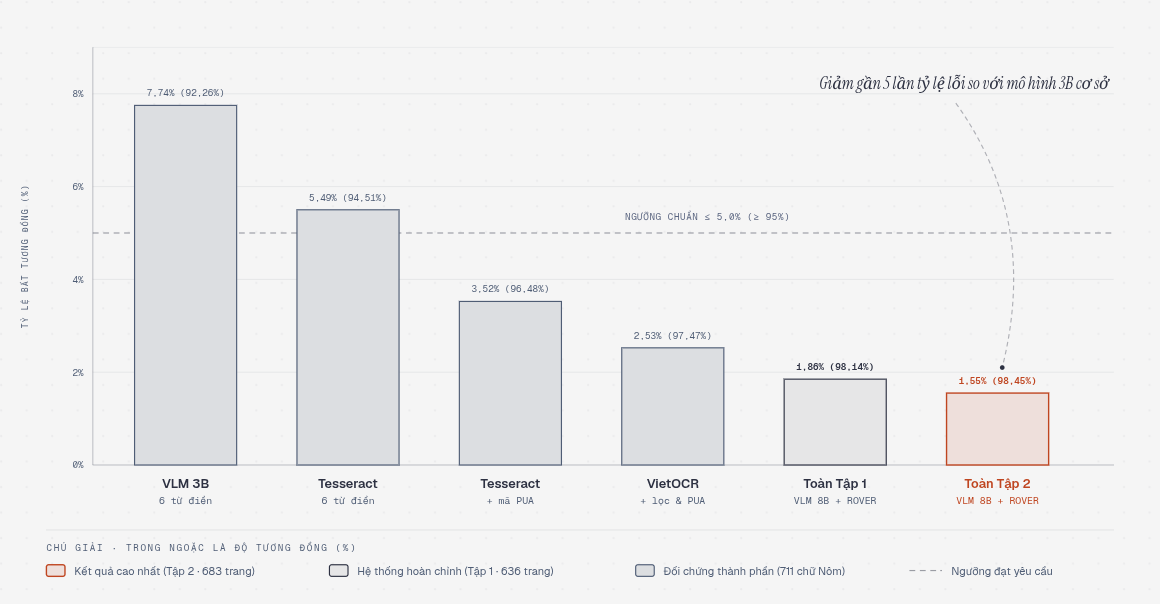
\includegraphics[width=0.95\linewidth]{images/fig3-benchmark.png}
    \caption{So sánh tỷ lệ bất tương đồng ngữ âm ($100\% - \text{Độ tương đồng}$) qua các cấu hình nhận dạng và chuẩn hóa}
    \label{fig:benchmark}
\end{figure}

\subsection{Phân tích định tính và phân rã phần dư sai khác}

Để minh họa rõ cách cơ chế ROVER liên ngôn ngữ xử lý các lỗi dấu vi mô trên dữ liệu thực tế, có thể xét một đoạn câu mang mật độ cao từ cổ và phụ âm dễ nhầm lẫn. Ở lượt đọc chính $48\text{ px}$, mô hình thị giác trả về chuỗi \textit{``Vì \textbf{chúng}, \textbf{dàng} ấy \textbf{Dấng}\ldots''}, mắc ba lỗi quen thuộc gồm nhầm \textit{ư} thành \textit{u} (tạo thành từ hiện đại \textit{chúng} vốn đúng chính tả tiếng Việt nên bộ soát lỗi đơn ngữ không phát hiện được) cùng hai lỗi mất nét ngang chữ \textit{đ} ở \textit{dàng} và \textit{Dấng}. Trong khi đó, bản đọc phụ lại nhận đúng ba từ trên nhưng đọc nhầm dấu mũ ở từ \textit{ấy}, cho ra chuỗi \textit{``Vì \textbf{chưng}, \textbf{đàng} \textbf{áy} \textbf{Đấng}\ldots''}. Khi đối chiếu với tập khóa ngữ âm trích xuất từ trang Hán Nôm đối ứng vốn có mặt các tự hình \nom{蒸} (\textit{chưng}), \nom{塘} (\textit{đàng}), \nom{等} (\textit{đấng}) và \nom{意} (\textit{ấy}), thuật toán ghi nhận khóa \code{chung}, \code{dang}, \code{dâng} không khớp tự hình nào trong vùng trang còn \code{chưng}, \code{đang}, \code{đâng} đều có đối ứng trực tiếp, nên chọn thay thế thành \textit{chưng}, \textit{đàng} và \textit{Đấng}. Ngược lại, tại vị trí \textit{ấy / áy}, khóa \code{ây} của bản chính đã khớp với chữ \nom{意} nên hệ thống giữ nguyên \textit{ấy}, tránh để sai sót từ bản phụ lan ngược vào kết quả cuối. Qua đó, câu hợp nhất đạt dạng đúng \textit{``Vì chưng, đàng ấy Đấng\ldots''} mà không một luồng đơn lẻ nào tự tạo ra được.

Bên cạnh các trường hợp được xử lý tốt, việc phân tích $2.479$ phần tử bất tương đồng còn lại trên tổng số $145.787$ tự hình tính điểm (tương ứng $1{,}86\%$ ở Tập 1 và $1{,}55\%$ ở Tập 2) cho thấy phần dư sai khác không xuất phát từ lỗi trượt ranh giới câu mà tập trung vào bốn nguyên nhân mang tính đặc thù của tư liệu lịch sử. Khoảng $45\%$ số lỗi còn lại đến từ sự thoái hóa vật lý cục bộ của bản khắc và mực in, chẳng hạn vết mọt giấy, chấm mực loang hoặc nét khắc bị gãy riêng lẻ trên từng chữ đơn khiến mô hình Hán Nôm đọc sang một chữ Hán khác bộ thủ mà không tạo thành quy luật lặp lại đủ đều để đưa vào bảng hiệu chỉnh tất định. Khoảng $25\%$ số lỗi bắt nguồn từ những biến thể dịch thuật vi mô ngay trong văn bản dịch âm 1--1, khi dịch giả đầu thế kỷ XX thỉnh thoảng thêm một hư từ tiếng Việt để câu văn tự nhiên hơn hoặc gom hai chữ Hán đẳng lập thành một từ đơn Quốc ngữ. Khoảng $25\%$ tiếp theo liên quan đến biến âm lịch sử và cách đọc địa phương thế kỷ XIX--XX xuất hiện rải rác chưa có trong bảy bộ từ điển chuẩn hóa, cùng một số rất ít tự hình lạ chưa có mục từ (trên toàn bộ $146.277$ chữ chỉ còn ba tự hình chưa có trong kho từ điển là \nom{䦕}, \ids{蔶} ở Tập 1 và \nom{𨢄} ở Tập 2). Phần nhỏ còn lại (khoảng $5\%$ tính chung các trường hợp ngoại lệ về mã hóa và ký tự hiếm) bao gồm tự hình Nôm ngoài chuẩn Unicode \nom{〓} (\ids{⿱}\nom{𥫗頓}, âm \textit{lớn}) được giữ nguyên trạng thái đánh dấu đỏ và truy vết tọa độ riêng nhằm đảm bảo tính trung thực về mặt văn bản học.
